
\documentclass[UTF8]{ctexart}
\usepackage{lmodern}
\usepackage{amsmath}
\usepackage{amssymb}
\usepackage{graphicx}
\usepackage{xcolor}
\usepackage{geometry}
\usepackage{tikz}
\usepackage{caption}
\usepackage{float}
\usepackage{pgfplots}
\usepackage{mathtools}
\geometry{left=2.18cm,right=2.18cm,top=1.54cm,bottom=2.0cm}
\pagestyle{empty}
\pgfplotsset{compat=1.18}
\title{\textbf {2025春计算方法--实验报告 \#3}}
\author{姓名:\underline{~~~~~~~~~~~}  学号:\underline{~~~~~~~~~~~~~~~~~} }
\date{\today}


\begin{document}


\maketitle

运行环境:\underline{~~~~~~~~~~~~}

\section*{实验内容与要求}


分别编写 Newton 迭代法 (通常也称 Newton-Raphson 迭代法)
\[\color{blue}x_{n+1}=x_n-\frac{f(x_n)}{f'(x_n)}\]
和霍氏迭代法
 \[\color{blue} x_{n+1}= x_n - \frac{2f(x_n)f'(x_n)}{2f'(x_n)f'(x_n) - f(x_n)f''(x_n)}, \, n=0,1,2,\cdots\]
的通用程序, 并利用它们对如下非线性方程
\[\color{blue} f(x)\coloneqq{\arctan(x)}+0.2x\sin\left(\dfrac x2\right)+0.601958 =0\]
求根,计算中的停止条件为$\color{blue}|f(x_n)|<10^{-8}$或迭代步数~$\color{blue}n>10^4$(可视为迭代失败).
\textbf{提示}:编程前分别手算出$~\color{blue}f'(x), f''(x)$。

\begin{itemize}
    \item 列表给出两种迭代方法在初始点 $x_0$ 依次取值$-75, -60,-50, -40, -30, -20, -10, -5, 0, 6, 15, 25, 35,$ $ 45, 50, 60, 75$时的迭代步数(若迭代步数超过1万步,可视为迭代失败)以及相应的数值解~$x_n$~(保留小数点后6位; 迭代失败时无需给出);
    \item 比较并分析两种方法的优劣,给出合理的算法分析并作实验小结。
\end{itemize}

\begin{figure}[H]
    \begin{center}
        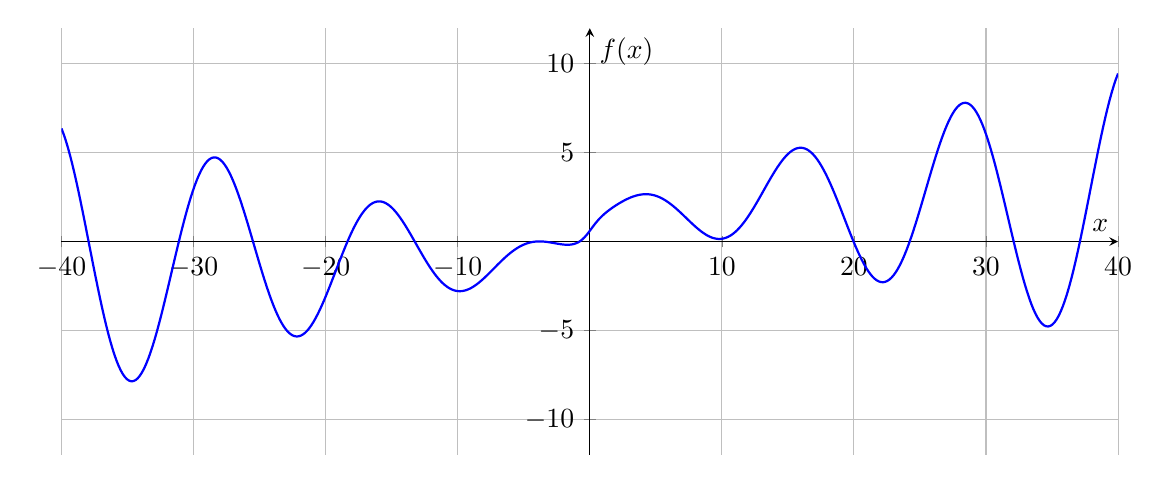
\begin{tikzpicture}
            \begin{axis}[
              xlabel={$x$},
              ylabel={$f(x)$},
              domain=-40:40,
              samples=500,
              axis lines=middle,
              xmin=-40, xmax=40,
              ymin=-12, ymax=12,
              grid=both,
              width=15cm,
              height=7cm,
            ]
            \addplot[blue, thick] { (pi/180)*atan(x) + 0.2*x*sin(deg(x/2)) + 0.601958 };
            \end{axis}
        \end{tikzpicture}
        \caption{函数图像}
        \label{fig:fig1}
    \end{center}
\end{figure}


\clearpage

\section{数值结果(列表或作图)}
\begin{table}[H]
\centering
\caption{实验结果: 误差精度~$\varepsilon = 10^{-8}$, 最大迭代步数为$10^4$}\begin{tabular}{ccccc}
\hline
Newton步数 & 数值解 & \color{blue}{初始点} & 霍氏步数 & 数值解 \\
\hline
\\
\hline
\end{tabular}
\label{tab:tab1}
\end{table}


\section{算法分析}


\section{实验小结}



\end{document}
